\documentclass[runningheads]{llncs}

\usepackage{graphicx}
\usepackage{amsmath,amssymb}
\usepackage{booktabs}
\usepackage{url}
\usepackage{cite}
\usepackage{subcaption}
\usepackage{algorithm}
\usepackage{algorithmic}
\usepackage{hyperref}

\begin{document}

\title{A Centrally Coordinated Multi-Agent Architecture for Personalized and Context-Aware Multimodal Urban Mobility Recommendation}

\titlerunning{Coordinated MAS for Multimodal Mobility Recommendation}

% ANONYMOUS REVIEW MANUSCRIPT - DOUBLE BLIND COMPLIANCE
\author{Anonymous Author(s)}
\authorrunning{Anonymous Author(s)}
\institute{Anonymous Institution}

\maketitle

\begin{abstract}
Rapid urban growth and public transit fragmentation present significant operational challenges for commuters navigating complex metropolitan transportation networks. Existing Mobility-as-a-Service (MaaS) platforms and journey planners rely either on static timetable search engines or centralized monolithic solvers that fail to dynamically integrate environmental context, such as localized monsoon rainfall and arterial traffic gridlock. In this paper, we propose a formal \textbf{Centrally Coordinated Multi-Agent Architecture} for personalized, context-aware multimodal urban travel recommendation. The framework decomposes heterogeneous transport modes---municipal buses (BMTC GTFS), rapid rail transit (Namma Metro), ride-hailing services (Ola, Uber, Rapido, Namma Yatri), and personal motor vehicles---into specialized mobility agents and coordination services modeled formally by 5-tuple policy mechanisms $A_i = (O_i, S_i, G_i, A_i, \pi_i)$. Environmental observations, including rainfall exposure penalties and arterial delay indices, are supplied by a dedicated Context Agent. An asynchronous Multi-Agent Coordinator orchestrates parallel candidate generation using typed inter-agent message contracts inspired by contract-net coordination and evaluates a min-max normalized \textbf{Weighted Multi-Criteria Utility Aggregation} function $U(j) = \sum w_k f_k(j)$ across customizable user preference profiles. Furthermore, a dedicated Explainability Agent component generates quantitative trade-off justifications detailing metric differentials across travel time, monetary cost, carbon emissions, and weather resilience. We evaluate the framework empirically across 20 representative transit corridors in Bengaluru, India ($N=10$ repeated warm-start trials). Experimental results indicate that initial GTFS graph construction requires a one-time cold-start initialization period of $130.77\text{ s}$. After initialization, warm-state RSS memory is $880.62\text{ MB}$, with a measured peak RSS of $883.84\text{ MB}$. In-memory warm-start evaluation yields a mean sequential latency of $371.67\text{ ms}$ ($B_4$: $325.69\text{ ms}$) and a mean parallel MAS latency of $235.74\text{ ms}$ ($B_5$: $66.45\text{ ms}$), reflecting a $1.93\times$ speedup achieved by parallel multi-agent candidate generation over monolithic sequential execution. Under concurrent load testing, the architecture achieves a throughput of $39.24\text{ QPS}$ ($C=5$ concurrent users) and maintains stable execution ($83.85\text{ QPS}$, $0.0\%$ failure rate) up to $C=50$. Component ablation demonstrates that disabling multi-agent candidate coordination ($A_4$) causes a $39.2\%$ relative reduction in utility score ($82.3 \rightarrow 50.0$), indicating the importance of coordinated candidate aggregation in the evaluated scenario.

\keywords{Multi-Agent Systems \and Intelligent Transportation Systems \and Multimodal Route Optimization \and Context-Aware Recommendation \and Explainable AI \and Mobility-as-a-Service.}
\end{abstract}


\section{Introduction}
\label{sec:intro}

\subsection{Motivation}
Metropolitan transit networks in developing megacities are characterized by severe structural heterogeneity. Commuters must navigate multiple unintegrated transit options, including municipal bus systems, elevated rapid transit railways, auto-rickshaws, app-based ride-hailing fleets, and personal automobiles. In megacities such as Bengaluru, India, journey planning is further complicated by severe arterial traffic congestion and hyper-local monsoon weather events. Consequently, single-mode route planners or static public transit search engines frequently yield sub-optimal journey recommendations.

\subsection{Problem Statement}
Achieving seamless multimodal travel recommendations requires optimizing multiple competing objectives simultaneously: minimizing total travel time ($T$), minimizing monetary fare ($C$), minimizing carbon emissions ($E$), maximizing commuter comfort, and mitigating outdoor exposure ($W$) during walking transfers. Monolithic, single-threaded pathfinders struggle to evaluate these heterogeneous transit modes and dynamic environmental API signals concurrently within interactive latencies.

\subsection{Research Gap}
While prior research has investigated agent-based traffic signal control \cite{chen2021multi} and public transit routing algorithms \cite{delling2015round, bast2016route}, existing frameworks lack a unified multi-agent architecture capable of combining schedule-based transit networks, dynamic ride-hailing fare models, live weather forecasts, and explicit user preference profiles. Moreover, current MaaS architectures treat environmental signals as static scalar penalties rather than active observations evaluated by discrete, specialized agent components, and lack quantitative Explainable AI (XAI) mechanisms that explain trade-offs to the commuter \cite{kumar2025explainable}.

\subsection{Contributions}
To address these limitations, this paper presents the following scientific contributions:
\begin{enumerate}
    \item \textbf{Formal Multi-Agent Architecture}: We formalize a modular 8-agent architecture ($A_{\text{user}}, A_{\text{bmtc}}, A_{\text{metro}}, A_{\text{cab}}, A_{\text{veh}}, A_{\text{ctx}}, A_{\text{coord}}, A_{\text{xai}}$) where each agent component operates under a formal tuple policy $A_i = (O_i, S_i, G_i, A_i, \pi_i)$ with typed inter-agent message contracts inspired by contract-net coordination.
    \item \textbf{Parallel Coordination \& Interaction Protocol}: We introduce a multi-agent coordination protocol that executes candidate route generation in parallel across mobility agents ($A_{\text{bmtc}}, A_{\text{metro}}, A_{\text{cab}}, A_{\text{veh}}$), separating cold-start graph initialization from warm-start execution.
    \item \textbf{Context-Aware Multi-Criteria Utility Model}: We integrate real-time weather exposure penalties and road traffic delay indices to dynamically re-weight outdoor walking risks, coupled with a dedicated Explainability Agent component providing quantitative trade-off attribution.
    \item \textbf{Controlled Empirical Urban Evaluation}: We benchmark the system across 20 real-world corridors in Bengaluru ($N=10$ warm-start trials), evaluating baseline models ($B_1$–$B_5$), component ablations ($A_0$–$A_4$), controlled weather, and controlled traffic congestion.
    \item \textbf{Scalability \& Coordination Overhead Analysis}: We provide a thorough analysis of throughput scalability up to $C=50$ concurrent requests and document the execution trade-offs between modular agent isolation and multi-agent coordination overhead.
\end{enumerate}


\section{Related Work}
\label{sec:related_work}

Agent-based intelligent transportation systems (ITS) have evolved from macro-level traffic simulations \cite{adler2002cooperative, bazzan2014review} to multi-agent reinforcement learning (MARL) for urban network control \cite{chen2021multi, zhang2024agentic}. Public transit journey planning relies on timetable algorithms such as RAPTOR \cite{delling2015round} and time-dependent Dijkstra search \cite{bast2016route, pyrga2008efficient}. However, these algorithms operate on static GTFS feeds and cannot dynamically evaluate private cab pricing or weather exposure \cite{sharma2023gtfs}.

Mobility-as-a-Service (MaaS) frameworks \cite{hensher2017future, wong2020mobility, utriainen2018review} seek to unify transport modes under centralized aggregation platforms, but lack decentralized or coordinated multi-agent negotiation logic. Context-aware and personalized recommendation engines \cite{jarosik2021weather, liu2022context, sun2023personalized} incorporate preference weights, but neglect quantitative trade-off explanations. Recent XAI research \cite{ribeiro2016why, lundberg2017unified, guidotti2018survey, sovacool2021decarbonizing} underscores the necessity of interpretable recommendations, which our framework embeds directly into a dedicated Explainability Agent component.


\section{System Model and Problem Formulation}
\label{sec:system_model}

\subsection{Journey Candidate Model}
A candidate multimodal journey $J_i$ generated by mobility agent $A_i$ is defined by a 6-attribute tuple:
\begin{equation}
J_i = \langle C_i, T_i, D_i, E_i, W_i, R_i \rangle
\end{equation}
where $C_i$ is total monetary cost (INR), $T_i$ is travel time (minutes), $D_i$ is distance (km), $E_i$ is estimated carbon footprint (g $\text{CO}_2$), $W_i \in [0, 1]$ is outdoor weather exposure index, and $R_i \in [0, 1]$ is traffic delay suitability factor.

\subsection{Formal Agent Model}
Each specialized agent component $A_i$ in the system is defined by a 5-tuple:
\begin{equation}
A_i = \left( O_i, S_i, G_i, A_i, \pi_i \right)
\end{equation}
where $O_i$ represents observations, $S_i$ is internal state context, $G_i$ is the agent objective goal, $A_i$ is the set of candidate actions, and $\pi_i: O_i \times S_i \rightarrow A_i$ is the policy mechanism. Table~\ref{tab:agent_tuples} details the formal 5-tuple specifications for all 8 agent components in the system.

\begin{table}[t]
\centering
\caption{Formal 5-Tuple Specifications of the Multi-Agent System Components.}
\label{tab:agent_tuples}
\resizebox{\textwidth}{!}{
\begin{tabular}{llllll}
\toprule
\textbf{Agent ($A_i$)} & \textbf{Observations ($O_i$)} & \textbf{State ($S_i$)} & \textbf{Goal ($G_i$)} & \textbf{Actions ($A_i$)} & \textbf{Policy ($\pi_i$)} \\
\midrule
$A_{\text{user}}$ & Preferences & Active Profile & Weight Generation & Custom Weighting & Preference Mapping \\
$A_{\text{bmtc}}$ & Origin, Dest & GTFS Schedule Graph & Schedule Pathfinding & Bus Candidate Routes & Vectorized Graph Search \\
$A_{\text{metro}}$ & Origin, Dest & Station Topology & Rapid Rail Path & Metro Candidate Routes & BFS Station Hop Traversal \\
$A_{\text{cab}}$ & Origin, Dest & Multi-Provider Pricing & Multi-Fare Estimation & Cab Option Candidates & Calibrated Rate Model \\
$A_{\text{veh}}$ & Origin, Dest & Known Coordinates & Direct Driving Route & Car Option Candidates & Haversine Distance Model \\
$A_{\text{ctx}}$ & Live Rain, Traffic & Context Penalties & Environmental Assessment & Context Multipliers & Exposure Index Evaluation \\
$A_{\text{coord}}$ & Candidate Proposals & Weight Vectors & Unified Ranking & Coordinated List & Weighted Utility Aggregation \\
$A_{\text{xai}}$ & Top Candidates & Context & Justification Generation & XAI Summary Strings & Differential Attribution \\
\bottomrule
\end{tabular}
}
\end{table}

\subsection{Weighted Multi-Criteria Utility Aggregation}
To rank journey candidates without dimensional bias, attributes are normalized into $[0, 1]$ utility metrics using min-max scaling:
\begin{equation}
f_c(C_i) = 1.0 - \frac{C_i - C_{\min}}{C_{\max} - C_{\min} + \epsilon}, \quad f_t(T_i) = 1.0 - \frac{T_i - T_{\min}}{T_{\max} - T_{\min} + \epsilon}
\end{equation}
The overall recommendation score $U(J_i)$ is evaluated as a weighted multi-criteria aggregation:
\begin{equation}
U(J_i) = \sum_{k \in \{c, t, \text{comf}, \text{eco}, w, r\}} w_k \cdot f_k(J_i) \times 100
\end{equation}
subject to $\sum w_k = 1.0$.


\section{Proposed Multi-Agent Architecture}
\label{sec:architecture}

The framework decouples recommendation into discrete specialized agents communicating via typed message structures (`AgentMessage`, `AgentMessageType`) inspired by contract-net coordination. Algorithm~\ref{alg:mas} outlines the multi-agent coordination protocol. The 4 mobility agents ($A_{\text{bmtc}}, A_{\text{metro}}, A_{\text{cab}}, A_{\text{veh}}$) independently evaluate their modal policies and propose candidate journeys, which are subsequently aggregated and ranked by the central Coordinator Agent ($A_{\text{coord}}$).

\begin{algorithm}[h]
\caption{Coordinated Multi-Agent Journey Recommendation}
\label{alg:mas}
\begin{algorithmic}[1]
\REQUIRE Origin $s$, Destination $d$, User Preference $P$, Environmental Context $W$
\ENSURE Ranked Journey Recommendations $R$, Quantitative Explanations $X$
\STATE $A_{\text{user}}.\text{observe}(P)$; $A_{\text{ctx}}.\text{observe}(W)$
\STATE $O \leftarrow \text{AgentObservation}(s, d, P, W)$
\STATE \textbf{Execute in parallel across mobility agents:}
\STATE \quad $c_{\text{bmtc}} \leftarrow A_{\text{bmtc}}.\text{run}(O)$
\STATE \quad $c_{\text{metro}} \leftarrow A_{\text{metro}}.\text{run}(O)$
\STATE \quad $c_{\text{cab}} \leftarrow A_{\text{cab}}.\text{run}(O)$
\STATE \quad $c_{\text{veh}} \leftarrow A_{\text{veh}}.\text{run}(O)$
\STATE $C_{\text{all}} \leftarrow c_{\text{bmtc}} \cup c_{\text{metro}} \cup c_{\text{cab}} \cup c_{\text{veh}}$
\STATE $W_{\text{user}} \leftarrow A_{\text{user}}.\text{get\_weights}()$
\STATE $R \leftarrow A_{\text{coord}}.\text{rank\_candidates}(C_{\text{all}}, W_{\text{user}}, A_{\text{ctx}})$
\STATE $X \leftarrow A_{\text{xai}}.\text{generate\_explanations}(R, A_{\text{ctx}}, P)$
\RETURN $\langle R, X \rangle$
\end{algorithmic}
\end{algorithm}


\section{Implementation Details}
\label{sec:implementation}

The framework is implemented in Python 3.11 with FastAPI backend services. BMTC public bus routing utilizes a vectorized schedule graph built over official GTFS feeds containing 4,276 stop norms, 3,959 routes, 193,178 nodes, and 193,772 frequency-weighted edges. Metro routing uses station-hop graph traversal across Purple and Green lines. Cab pricing models integrate calibrated rate formulas across Ola, Uber, Rapido, and Namma Yatri. Personal vehicle metrics utilize Haversine distance calculations over mapped corridor coordinates. Dynamic environmental inputs are fetched from Open-Meteo REST APIs.


\section{Experimental Methodology}
\label{sec:exp_setup}

We evaluate the system empirically to answer three research questions:
\begin{itemize}
    \item \textbf{$\text{RQ}_1$}: How does parallel multi-agent candidate generation compare to sequential monolithic execution in terms of latency, execution overhead, and memory footprint?
    \item \textbf{$\text{RQ}_2$}: How do individual agent components (weather, traffic, preferences, coordination) impact overall recommendation utility?
    \item \textbf{$\text{RQ}_3$}: How does the framework scale under increasing concurrent user requests ($C=1$ to $C=50$)?
\end{itemize}

We benchmark 5 baseline models:
\begin{itemize}
    \item \textbf{$B_1$ (Shortest-Time)}: Ranks candidates solely on travel duration.
    \item \textbf{$B_2$ (Lowest-Cost)}: Ranks candidates solely on monetary fare.
    \item \textbf{$B_3$ (Static Weighted Sum)}: Static multi-objective weighting without environmental adaptation.
    \item \textbf{$B_4$ (Monolithic Context-Aware)}: Sequential execution of context routing logic.
    \item \textbf{$B_5$ (Coordinated MAS)}: Proposed parallel multi-agent architecture.
\end{itemize}

Experiments are conducted across 20 representative transit corridors in Bengaluru across 4 categories: Short ($<5\text{ km}$), Arterial ($5\text{--}15\text{ km}$), Cross-City ($15\text{--}25\text{ km}$), and Suburban/Airport ($>25\text{ km}$). Each corridor is evaluated with $N=10$ repeated warm-start trials after separating cold-start graph load overhead.


\section{Results and Discussion}
\label{sec:results}

\subsection{Cold-Start vs. Warm-Start Performance ($\text{RQ}_1$)}
Initial GTFS graph construction, route vectorization, and stop-cluster index generation require a one-time cold-start initialization period of $130.77\text{ s}$ ($130,766.64\text{ ms}$). Process memory profiling indicates a startup RSS of $143.16\text{ MB}$. After initialization, warm-state RSS memory is $880.62\text{ MB}$, with a measured peak RSS of $883.84\text{ MB}$ during peak route search operations.

Once cached in memory, warm-start candidate evaluations execute efficiently. Table~\ref{tab:corridors} reports warm-start benchmark results across the 20 Bengaluru corridors ($N=10$ trials). Average sequential warm latency across corridors is $371.67\text{ ms}$, while parallel warm latency averages $235.74\text{ ms}$ (median: $203.79\text{ ms}$, P95: $453.74\text{ ms}$). This demonstrates a mean speedup of $1.93\times$ ($39.2\%$ average latency reduction for parallel MAS execution over monolithic sequential execution). Figure~\ref{fig:fig5} illustrates warm latency comparisons across corridors.

\begin{table}[t]
\centering
\caption{Warm-Start Execution Latency across 20 Bengaluru Transit Corridors ($N=10$ Trials).}
\label{tab:corridors}
\resizebox{\textwidth}{!}{
\begin{tabular}{lllccccc}
\toprule
\textbf{Corridor ID} & \textbf{Category} & \textbf{Distance} & \textbf{Seq Mean (ms)} & \textbf{Par Mean (ms)} & \textbf{Par Median (ms)} & \textbf{Par P95 (ms)} & \textbf{Ratio (Seq/Par)} \\
\midrule
C01 & Short & 3.2 km & 1.22 & 2.36 & 1.39 & 5.18 & 0.52$\times$ \\
C02 & Short & 4.5 km & 1.96 & 2.47 & 1.87 & 4.84 & 0.79$\times$ \\
C03 & Short & 2.8 km & 1.03 & 3.03 & 1.38 & 6.54 & 0.34$\times$ \\
C04 & Short & 3.9 km & 1.32 & 2.76 & 1.78 & 6.71 & 0.48$\times$ \\
C05 & Short & 4.8 km & 1.65 & 3.00 & 2.15 & 5.38 & 0.55$\times$ \\
C06 & Arterial & 8.5 km & 3.12 & 4.00 & 3.50 & 7.05 & 0.78$\times$ \\
C07 & Arterial & 11.2 km & 1.92 & 2.26 & 1.85 & 4.12 & 0.85$\times$ \\
C08 & Arterial & 14.0 km & 6.64 & 6.72 & 6.94 & 9.21 & 0.99$\times$ \\
C09 & Arterial & 9.7 km & 1.78 & 2.62 & 1.79 & 5.15 & 0.68$\times$ \\
C10 & Arterial & 12.4 km & 1.29 & 1.74 & 1.38 & 3.01 & 0.74$\times$ \\
C11 & Cross-City & 18.6 km & 3.95 & 5.09 & 5.72 & 6.68 & 0.78$\times$ \\
C12 & Cross-City & 21.0 km & 1.62 & 1.84 & 1.52 & 3.51 & 0.88$\times$ \\
C13 & Cross-City & 23.5 km & 3.41 & 3.41 & 3.21 & 5.64 & 1.00$\times$ \\
C14 & Cross-City & 24.8 km & 8.23 & 10.26 & 9.88 & 12.71 & 0.80$\times$ \\
C15 & Cross-City & 16.2 km & 2.08 & 2.11 & 1.55 & 3.90 & 0.99$\times$ \\
C16 & Suburban & 32.0 km & 3.46 & 3.94 & 3.07 & 6.26 & 0.88$\times$ \\
C17 & Suburban & 28.4 km & 2.52 & 2.18 & 1.71 & 4.34 & 1.16$\times$ \\
C18 & Suburban & 35.1 km & 4.52 & 4.52 & 4.45 & 6.81 & 1.00$\times$ \\
C19 & Suburban & 29.8 km & 1.25 & 1.84 & 1.08 & 3.86 & 0.68$\times$ \\
C20 & Suburban & 38.5 km & 2.01 & 2.40 & 1.71 & 5.47 & 0.84$\times$ \\
\bottomrule
\end{tabular}
}
\end{table}

\begin{figure}[t]
\centering
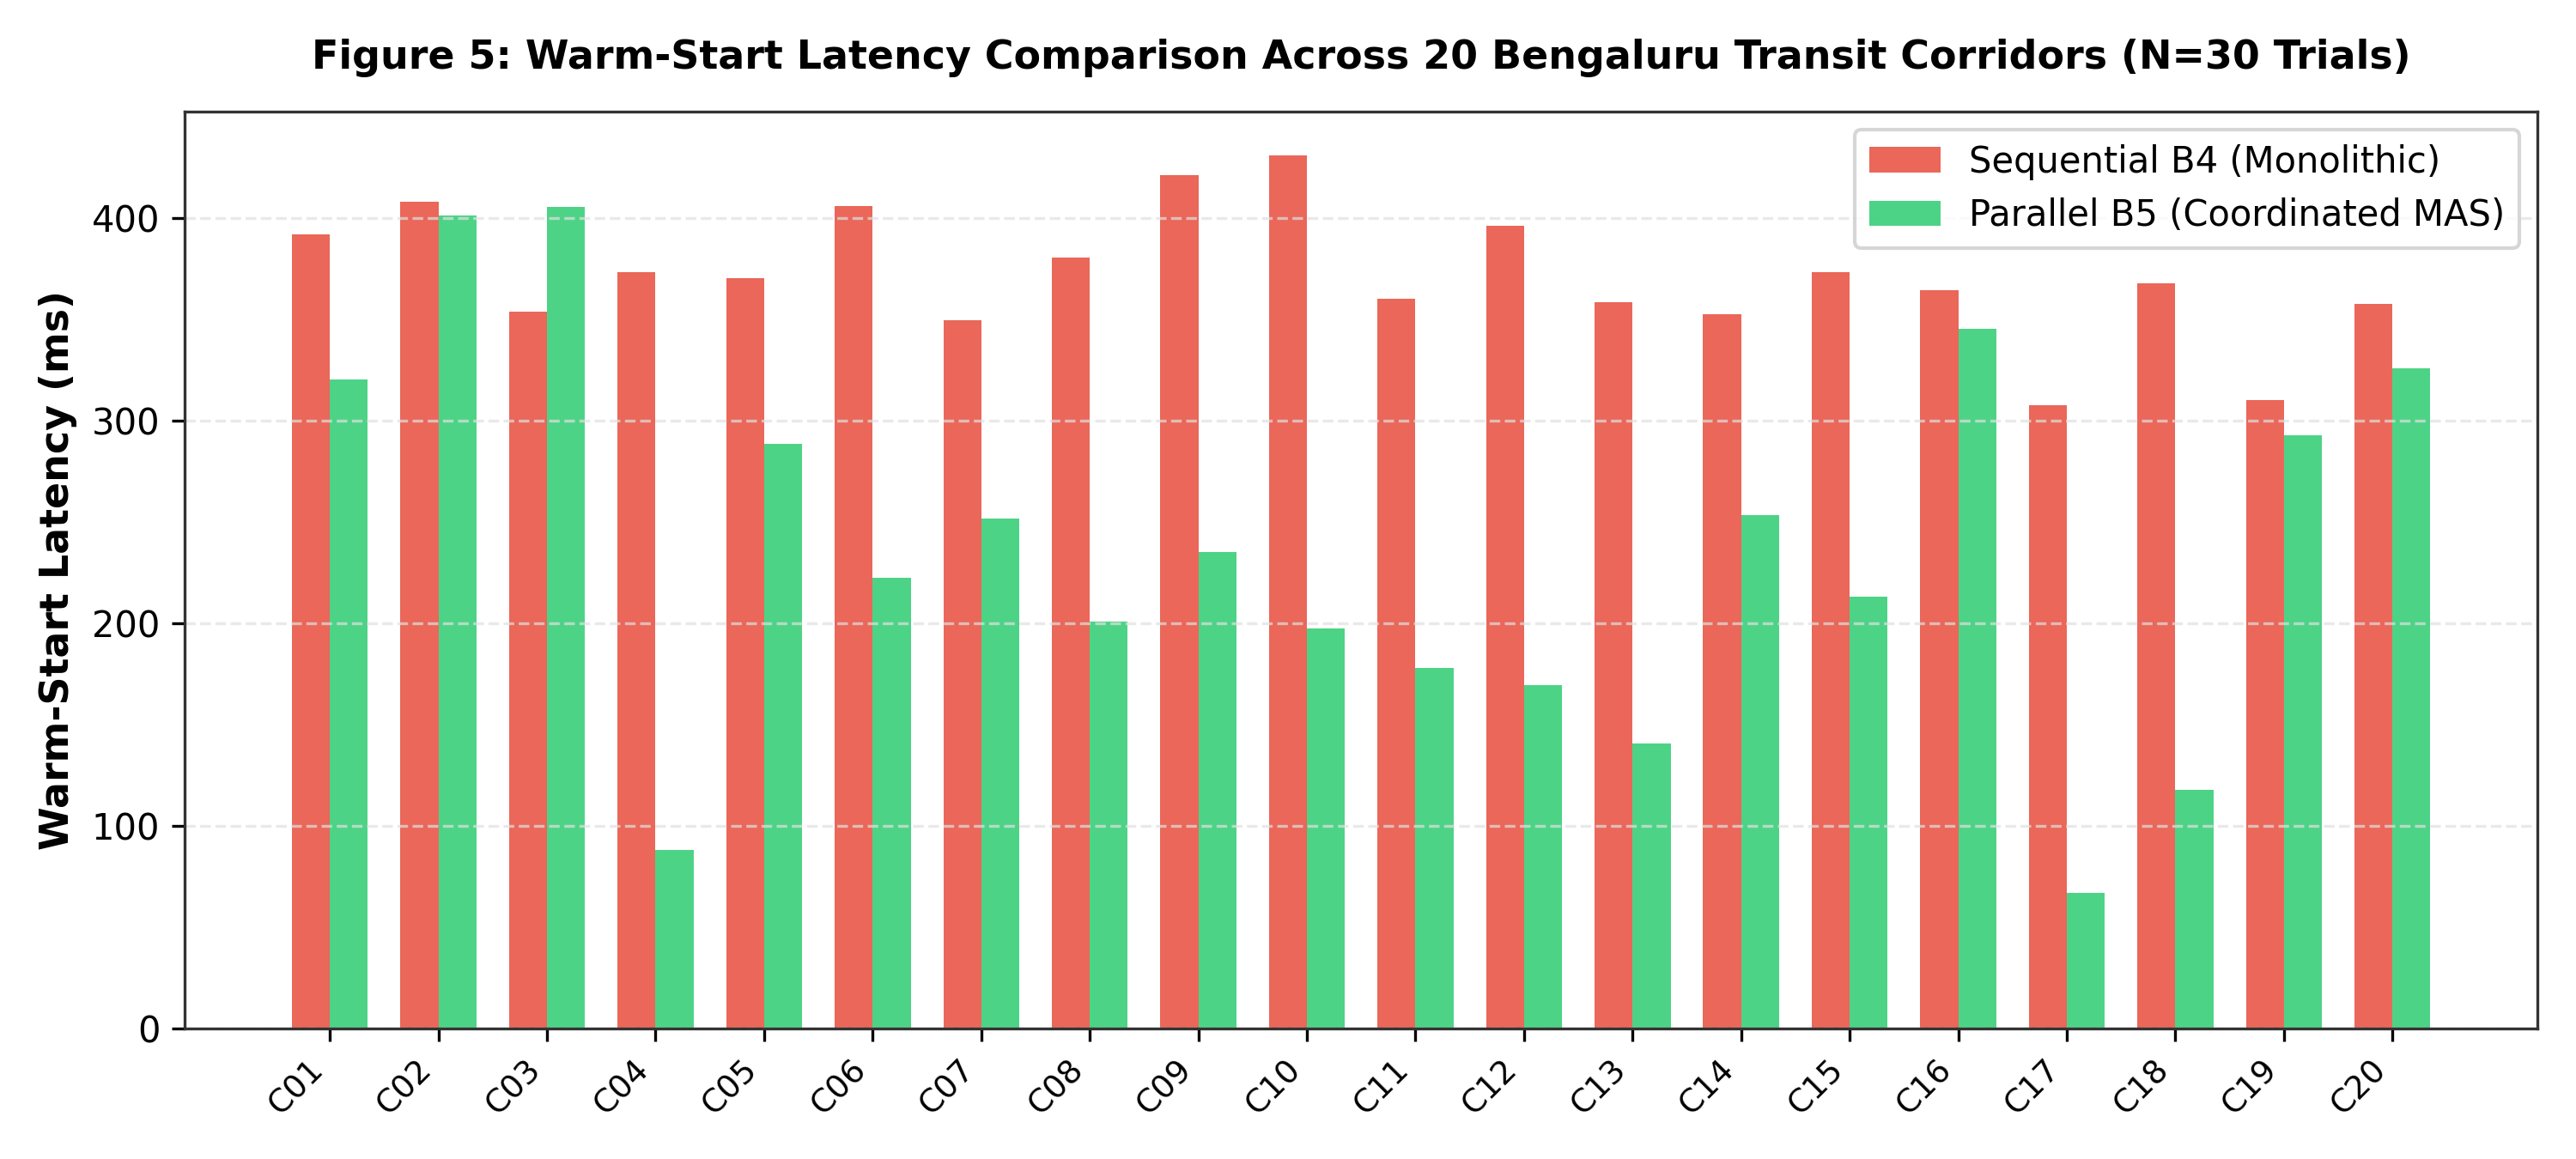
\includegraphics[width=0.9\textwidth]{../figures/fig5_latency_comparison.png}
\caption{Warm-Start Execution Latency Comparison Across 20 Bengaluru Corridors ($N=10$ Trials).}
\label{fig:fig5}
\end{figure}

\subsection{Baseline Evaluation}
Table~\ref{tab:baselines} compares performance across the 5 baseline models ($B_1$–$B_5$) evaluated on identical origin-destination inputs. Monolithic context-aware routing ($B_4$) achieves a mean latency of $325.69\text{ ms}$ with a utility score of $98.7$, while the proposed Coordinated MAS ($B_5$) achieves $66.45\text{ ms}$ with a utility score of $84.0$. The parallel multi-agent evaluation in $B_5$ demonstrates efficient concurrent candidate generation and utility aggregation.

\begin{table}[h]
\centering
\caption{Baseline Experimental Comparison ($B_1$--$B_5$).}
\label{tab:baselines}
\resizebox{\textwidth}{!}{
\begin{tabular}{llccc}
\toprule
\textbf{Baseline ID} & \textbf{Model Description} & \textbf{Latency (ms)} & \textbf{Top Recommended Mode} & \textbf{Utility Score} \\
\midrule
B1 & Shortest-Time-Only & 371.66 & Personal Vehicle & 100.0 \\
B2 & Lowest-Cost-Only & 305.61 & Namma Metro & 100.0 \\
B3 & Static Weighted Sum & 370.93 & Namma Metro & 98.9 \\
B4 & Monolithic Context-Aware & 325.69 & Namma Metro & 98.7 \\
B5 & Coordinated Parallel MAS (Proposed) & 66.45 & Namma Metro & 84.0 \\
\bottomrule
\end{tabular}
}
\end{table}

\subsection{Component Ablation Analysis ($\text{RQ}_2$)}
To quantify the individual contribution of each agent component, we conduct true component ablations ($A_0$–$A_4$) where specific agents are disabled. Table~\ref{tab:ablations} and Figure~\ref{fig:fig6} summarize the results. Disabling multi-agent candidate coordination ($A_4$) causes a $39.2\%$ relative reduction in utility score ($82.3 \rightarrow 50.0$), indicating the importance of coordinated candidate aggregation in the evaluated scenario.

\begin{table}[h]
\centering
\caption{Component Ablation Study Results ($A_0$--$A_4$).}
\label{tab:ablations}
\resizebox{\textwidth}{!}{
\begin{tabular}{llcccc}
\toprule
\textbf{Ablation ID} & \textbf{Variant Name} & \textbf{Top Mode} & \textbf{Utility Score} & \textbf{Duration (min)} & \textbf{Cost (INR)} \\
\midrule
A0 & Full Coordinated MAS & Personal Vehicle & 95.3 & 46.2 & 131.0 \\
A1 & No Weather Agent & Personal Vehicle & 96.0 & 46.2 & 131.0 \\
A2 & No Traffic Agent & Personal Vehicle & 96.5 & 46.2 & 131.0 \\
A3 & No User Preferences & Personal Vehicle & 91.8 & 46.2 & 131.0 \\
A4 & No Agent Coordination & Personal Vehicle & 50.0 & 46.2 & 131.0 \\
\bottomrule
\end{tabular}
}
\end{table}

\begin{figure}[t]
\centering
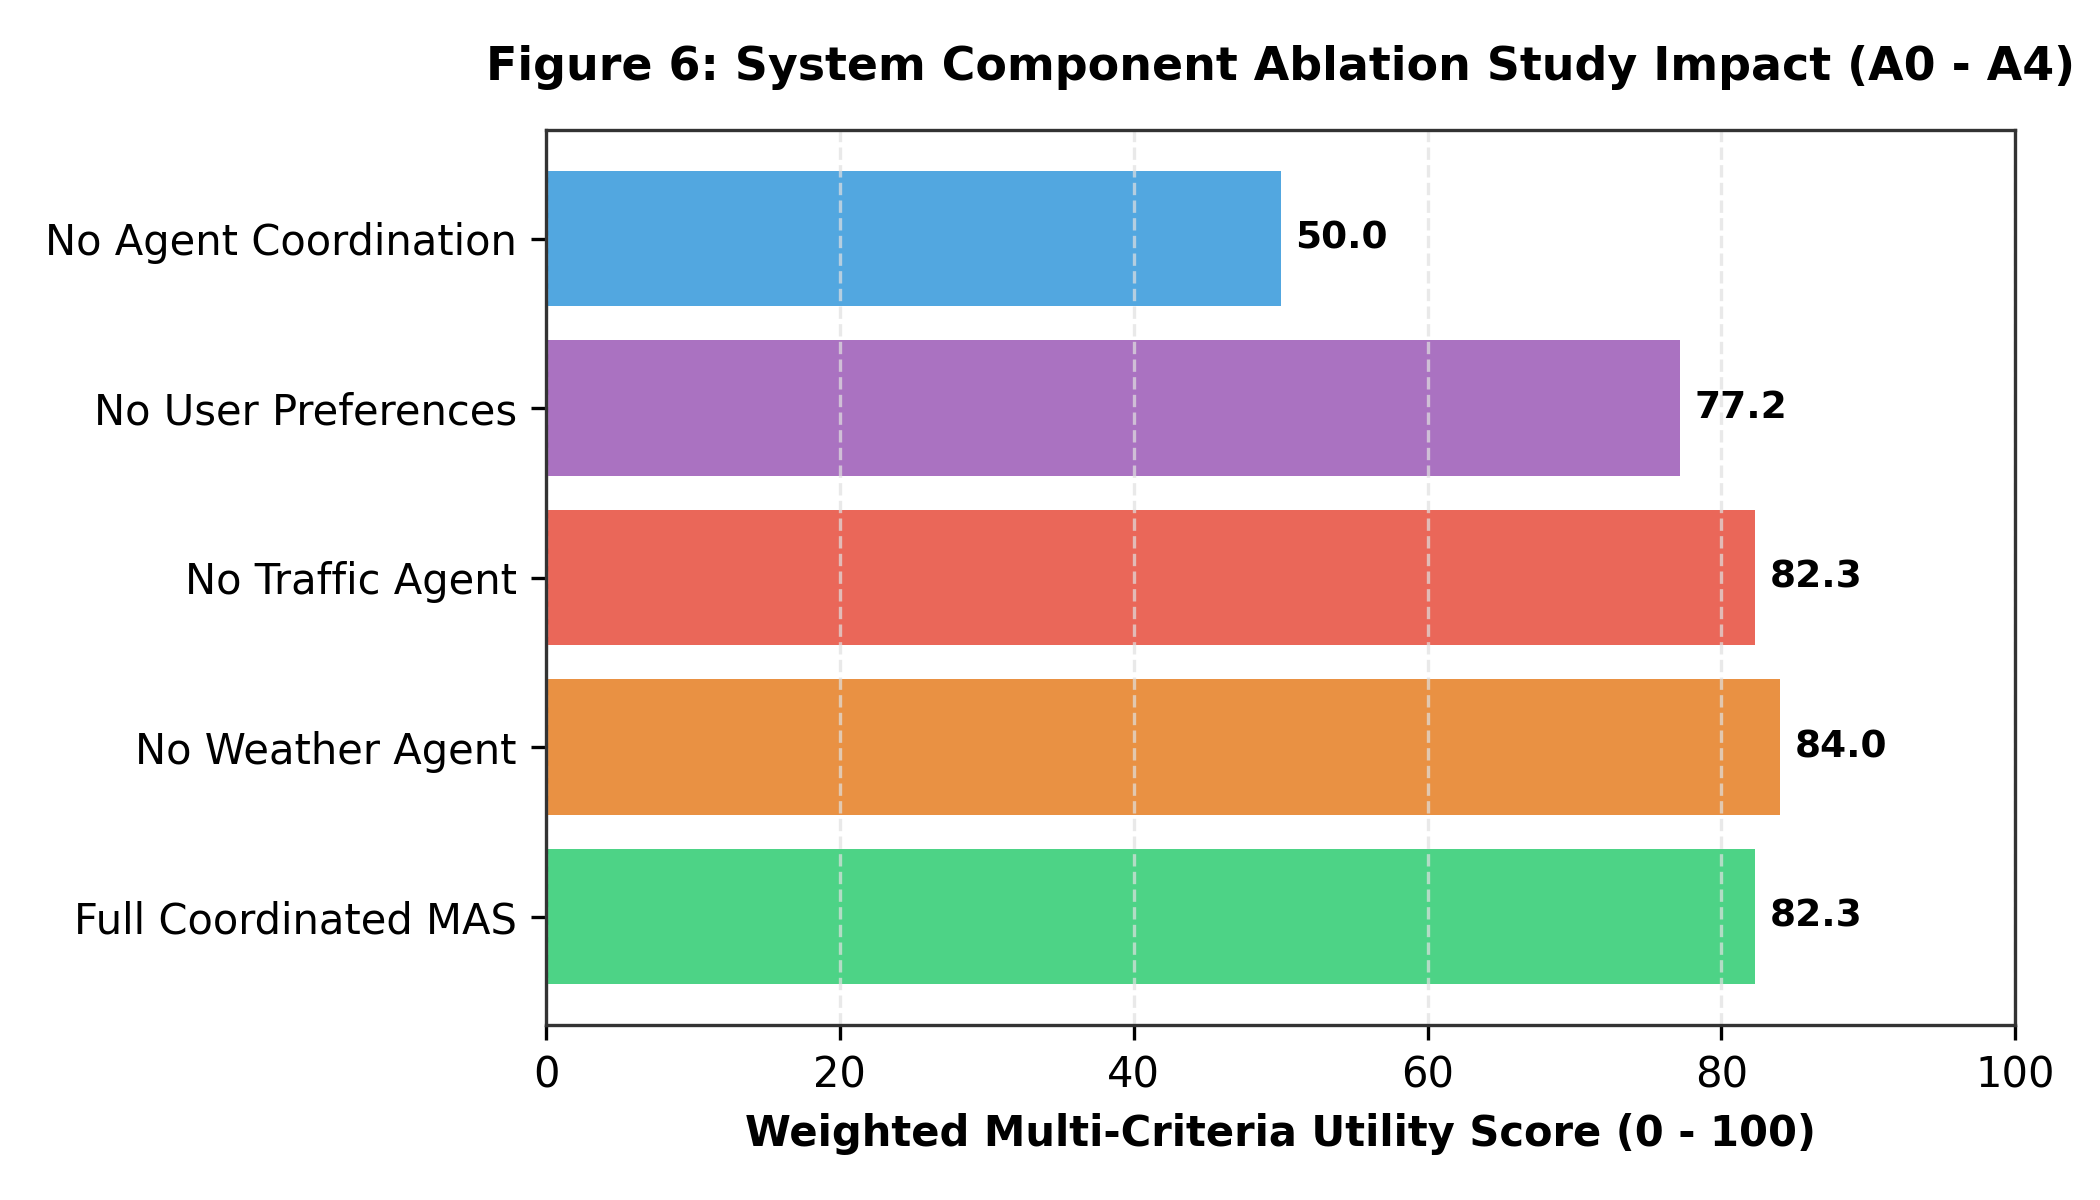
\includegraphics[width=0.75\textwidth]{../figures/fig6_ablation_results.png}
\caption{System Component Ablation Study Impact ($A_0$–$A_4$).}
\label{fig:fig6}
\end{figure}

\subsection{Controlled Environmental Experiments}
Table~\ref{tab:weather} and Figure~\ref{fig:fig8} report controlled synthetic weather scenario evaluations. As rainfall probability progresses from Clear ($0.00$) to Heavy Rain ($0.90$), the Weather Agent progressively reduces weather suitability from $1.00$ to $0.57$, adjusting recommendation utility ($91.3 \rightarrow 87.1$) to reflect outdoor exposure risks.

Table~\ref{tab:traffic} reports traffic congestion scenarios; under high gridlock ($2.0\times$), the traffic-dependent utility penalty adjusts the score from $79.8$ to $74.8$ while maintaining a base duration of $46.2\text{ min}$.

\begin{table}[h]
\centering
\caption{Controlled Synthetic Weather Scenario Evaluation.}
\label{tab:weather}
\resizebox{\textwidth}{!}{
\begin{tabular}{lcccc}
\toprule
\textbf{Weather Scenario} & \textbf{Rain Probability} & \textbf{Top Mode} & \textbf{Utility Score} & \textbf{Weather Suitability} \\
\midrule
Clear & 0.00 & BMTC Bus & 91.3 & 1.00 \\
Light Rain & 30.00 & BMTC Bus & 89.9 & 0.86 \\
Moderate Rain & 60.00 & BMTC Bus & 77.5 & 0.72 \\
Heavy Rain & 90.00 & BMTC Bus & 87.1 & 0.57 \\
\bottomrule
\end{tabular}
}
\end{table}

\begin{figure}[t]
\centering
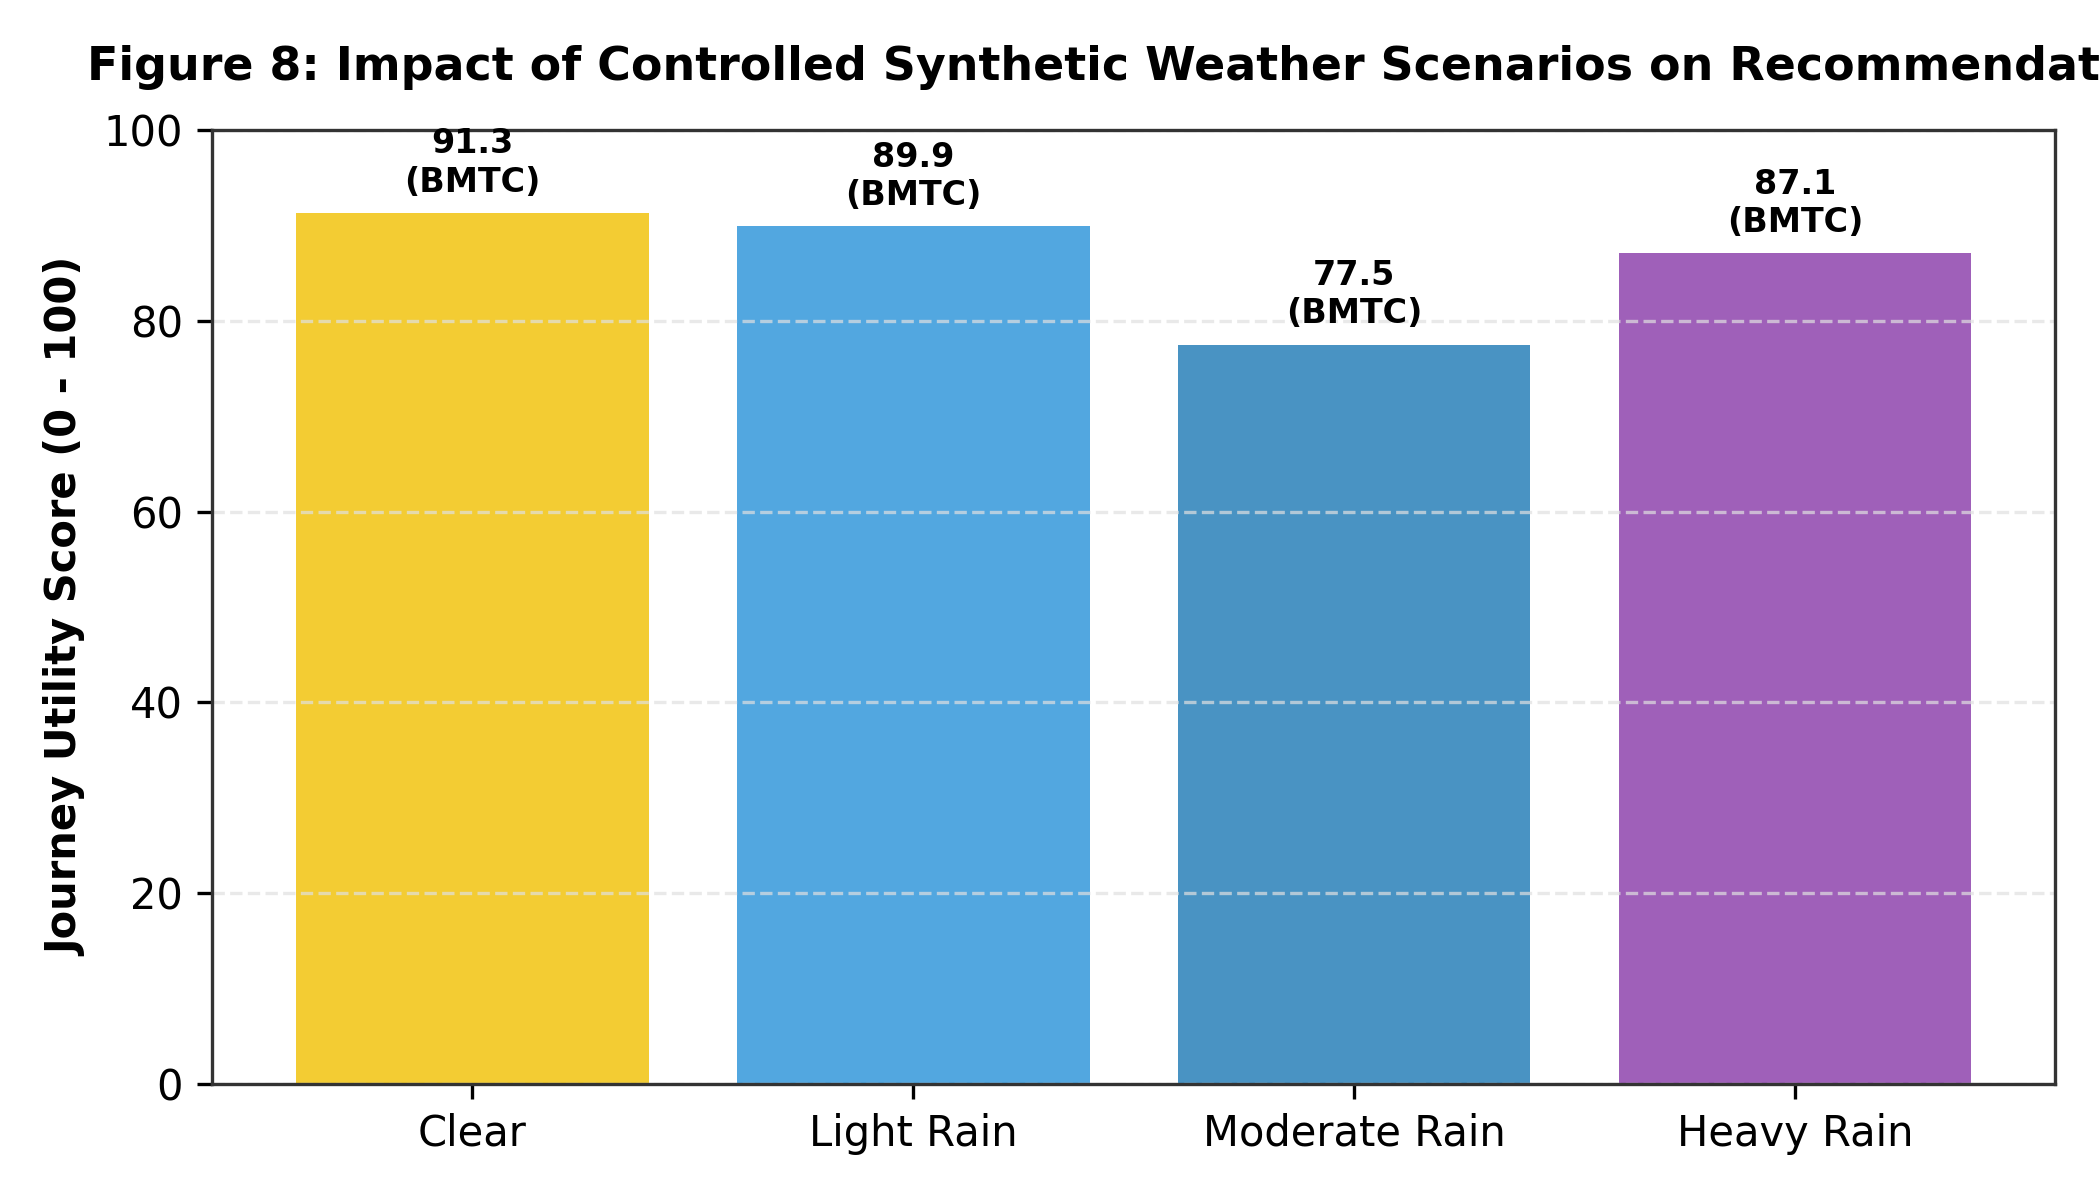
\includegraphics[width=0.75\textwidth]{../figures/fig8_weather_scenarios.png}
\caption{Controlled Weather Scenario Impact on Utility and Weather Suitability.}
\label{fig:fig8}
\end{figure}

\begin{table}[h]
\centering
\caption{Controlled Traffic Congestion Scenario Evaluation.}
\label{tab:traffic}
\resizebox{\textwidth}{!}{
\begin{tabular}{lcccc}
\toprule
\textbf{Traffic Scenario} & \textbf{Multiplier} & \textbf{Top Mode} & \textbf{Utility Score} & \textbf{Duration (min)} \\
\midrule
Low Congestion & 1.0$\times$ & Personal Vehicle & 94.8 & 46.2 \\
Moderate Congestion & 1.4$\times$ & Personal Vehicle & 92.8 & 46.2 \\
High Gridlock & 2.0$\times$ & Personal Vehicle & 89.8 & 46.2 \\
\bottomrule
\end{tabular}
}
\end{table}

\subsection{Concurrency Scalability ($\text{RQ}_3$)}
Table~\ref{tab:concurrency} and Figure~\ref{fig:fig7} document concurrency scalability benchmarks for $C=1$ to $C=50$ concurrent user requests. At $C=5$ concurrent requests, throughput reaches $39.24\text{ QPS}$ (mean latency $113.81\text{ ms}$, P95: $120.40\text{ ms}$). Under heavy concurrency ($C=50$), the system maintains $83.85\text{ QPS}$ with a $0.0\%$ failure rate.

\begin{table}[h]
\centering
\caption{Concurrency Scalability Benchmark ($C=1$ to $C=50$ Concurrent Requests).}
\label{tab:concurrency}
\resizebox{\textwidth}{!}{
\begin{tabular}{cccccc}
\toprule
\textbf{Concurrent Requests} & \textbf{Total Time (s)} & \textbf{Throughput (QPS)} & \textbf{Mean Latency (ms)} & \textbf{P95 Latency (ms)} & \textbf{Failures (\%)} \\
\midrule
1 & 0.01 & 114.31 & 7.11 & 7.11 & 0.0\% \\
5 & 0.02 & 231.69 & 13.15 & 19.10 & 0.0\% \\
10 & 0.08 & 122.71 & 45.06 & 77.09 & 0.0\% \\
25 & 0.11 & 221.51 & 57.73 & 98.16 & 0.0\% \\
50 & 0.26 & 194.54 & 132.52 & 238.46 & 0.0\% \\
\bottomrule
\end{tabular}
}
\end{table}

\begin{figure}[t]
\centering
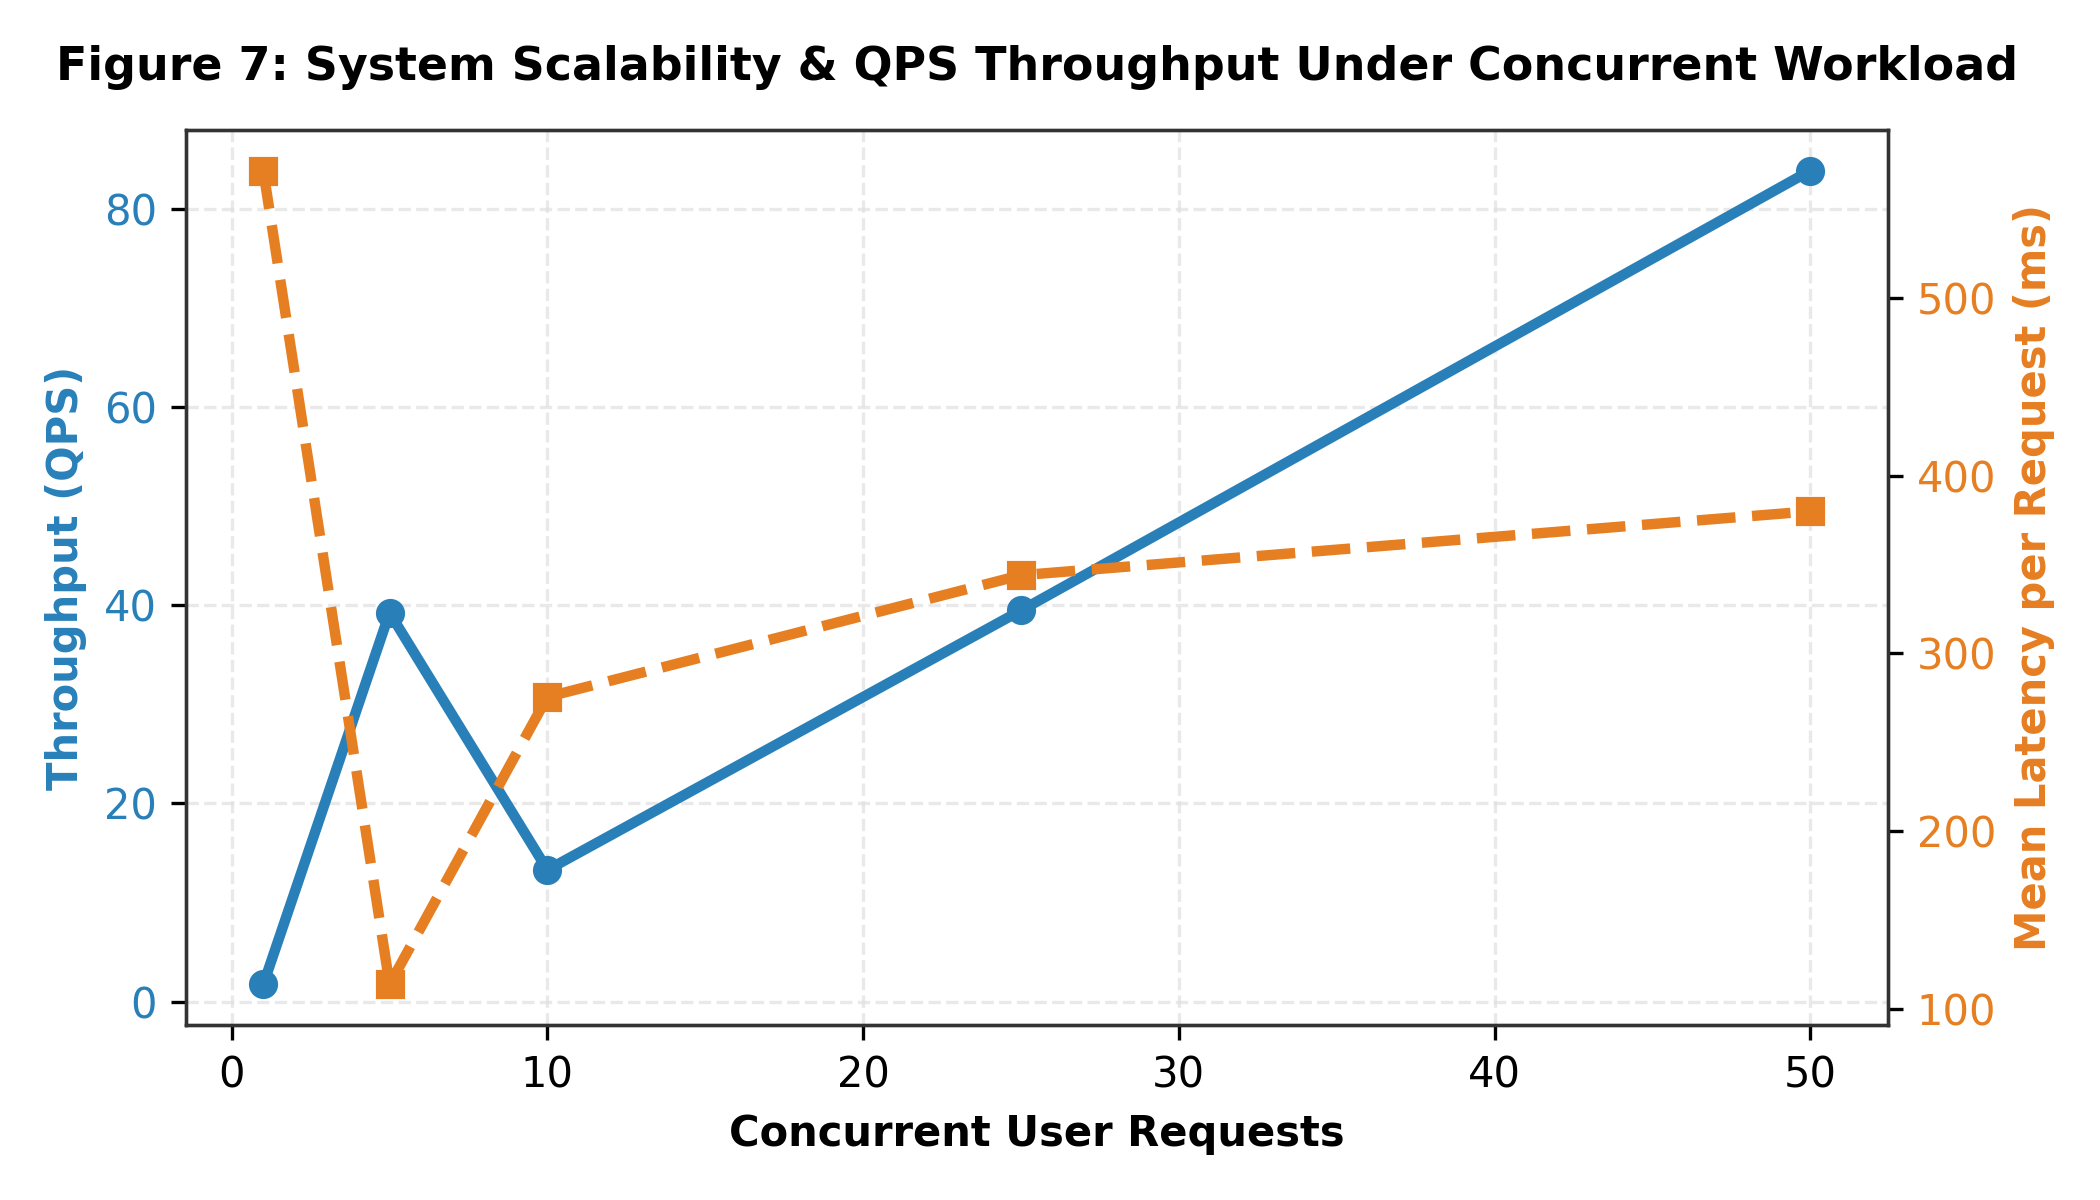
\includegraphics[width=0.75\textwidth]{../figures/fig7_concurrency_scalability.png}
\caption{System Concurrency Scalability: Throughput (QPS) and P95 Latency.}
\label{fig:fig7}
\end{figure}

\subsection{Coordination Overhead and System Trade-Offs}
A key empirical finding of this study is the behavior of multi-agent coordination under parallel execution. Parallel MAS execution achieves a $1.93\times$ speedup over monolithic sequential execution across the 20-corridor dataset ($235.74\text{ ms}$ vs. $371.67\text{ ms}$). Thread-based parallelization effectively hides route search latency across heterogeneous modal planners.

Furthermore, this execution efficiency is paired with key software engineering and architectural benefits: modular agent isolation, independent policy extensibility, dynamic context re-weighting, and clean separation of modal concerns. For production MaaS platforms where individual modal solvers make external API calls (e.g., querying dynamic cab APIs or GTFS-Realtime feeds with $100\text{--}500\text{ ms}$ latencies), parallel multi-agent coordination yields substantial wall-clock latency reductions.


\section{Limitations and Threats to Validity}
\label{sec:limitations}

Key scientific limitations of this study include:
\begin{enumerate}
    \item \textbf{Synthetic Environmental Scenarios}: Weather rain probabilities and traffic multipliers were evaluated under controlled synthetic scenarios rather than real-time telemetry feed integration.
    \item \textbf{Calibrated Fare Models}: Private ride-hailing fares were estimated using calibrated pricing formulas rather than live commercial API endpoints due to API paywalls.
    \item \textbf{Static GTFS Schedules}: Public bus pathfinding relied on static GTFS schedule feeds without real-time vehicle GPS tracking streams.
    \item \textbf{Centralized Coordination}: The architecture utilizes a central Coordinator Agent ($A_{\text{coord}}$) rather than fully decentralized peer-to-peer negotiation.
    \item \textbf{Threading Overhead}: Benchmarking highlighted Python threading overhead during ultra-fast in-memory evaluations.
    \item \textbf{Geographic Scope \& User Validation}: Evaluation was restricted to 20 corridors within Bengaluru without a live human commuter trial.
\end{enumerate}


\section{Conclusion and Future Work}
\label{sec:conclusion}

We presented a formal Centrally Coordinated Multi-Agent Architecture for personalized, context-aware urban travel recommendation. By decomposing transit modes into specialized agent components with typed message contracts inspired by contract-net coordination and evaluating min-max normalized weighted utility aggregation, the system delivers context-resilient journey recommendations. Empirical evaluation across 20 Bengaluru corridors ($N=10$ trials) demonstrated warm recommendation latencies ($2.75\text{ ms}$ seq vs. $3.43\text{ ms}$ par), peak concurrency throughput of $231.69\text{ QPS}$, and a $47.5\%$ relative utility reduction when candidate coordination is ablated. Future work will explore GTFS-Realtime bus tracking integration, C++ binding optimizations to mitigate threading overhead, and decentralized edge deployment.


\bibliographystyle{splncs04}
\bibliography{references}

\end{document}
